\documentclass[10pt,twocolumn,letterpaper]{article}

\usepackage{cvpr}
\usepackage{times}
\usepackage{epsfig}
\usepackage{graphicx}
\usepackage{amsmath}
\usepackage{amssymb}
\usepackage{mathtools}
\usepackage{array}
\usepackage{multirow}
\usepackage{float}


% Include other packages here, before hyperref.

% If you comment hyperref and then uncomment it, you should delete
% egpaper.aux before re-running latex.  (Or just hit 'q' on the first latex
% run, let it finish, and you should be clear).
\usepackage[breaklinks=true,bookmarks=false]{hyperref}

\cvprfinalcopy % *** Uncomment this line for the final submission

\def\cvprPaperID{****} % *** Enter the CVPR Paper ID here
\def\httilde{\mbox{\tt\raisebox{-.5ex}{\symbol{126}}}}


% Pages are numbered in submission mode, and unnumbered in camera-ready
%\ifcvprfinal\pagestyle{empty}\fi
\setcounter{page}{1}
\begin{document}

%%%%%%%%% TITLE
\title{Using Gated Recurrent Unit (GNU) Neural Networks to predict next day and intraday Google Stock prices}

\author{Julian Cabezas Pena Student ID: a1785086\\
Assignment 3. Deep Learning Fundamentals, 2020 \\
University of Adelaide\\
{\tt\small julian.cabezaspena@student.adelaide.edu.au}
% For a paper whose authors are all at the same institution,
% omit the following lines up until the closing ``}''.
% Additional authors and addresses can be added with ``\and'',
% just like the second author.
% To save space, use either the email address or home page, not both
}

\maketitle
%\thispagestyle{empty}

%%%%%%%%% ABSTRACT
\begin{abstract}
	
The prediction of stock prices is one of the biggest challenges in the field of time series prediction. In the last decade, the use of Recurrent Neural Networks (RNN) has appeared like a suitable tool for this purpose, given the nature of this kind of architectures to deal with sequences of data, such as stock time series. In this paper, the use of a RNN architecture based in Gated Recurrent Units (GRU) is tested to predict the Open, High, Low and Close price of the Google stock, along with its trading volume, testing models to predict next day values (including and excluding the volume), and prices in the same day (intraday) given the Open price. The results show that the inclusion of the Open price of the same day greatly increase the prediction performance of the models, reaching a RMSE of 3.9610 in the case of the Low price a RMSE of 4.5980 in the High price. The resulting models can provide insights in the decision making of the traders, but can not be used as sole input This research showed the difficulty of the prediction of stock prices and showed the importance of the correct choosing of input and output variables.

\end{abstract}

%%%%%%%%% BODY TEXT
\section{Introduction}

The prediction of stock prices in the future is a topic that has attracted both academic and industry investigators \cite{Zhao2020}, and is it often considered as one of the most challenging problems in the field of time series prediction \cite{Kara2011}. Given the high volatility, complexity and non-linearity of the stock market, trading can not rely on the trader's intuition or experience, making the use of machine learning methods a research hotspot \cite{Qiu2020}.

In the last years, one of the methods that has been more frequently used to predict stock prices is the use of Recurrent Neural Networks (RNN). These kind of neural network architectures deal with the problem of varying dimensionality, processing sequences of input data of varying length, and are commonly used in language and audio processing \cite{Skansi2018}, while also being suitable for time series prediction \cite{Zhao2020}. While other architectures such as the convolution neural networks or the multi layer perceptron present connections that push the information forward, Recurrent Neural Networks also contain connections that bring the information backward to a layer as an input \cite{Skansi2018}.

Nowadays, the most commonly used Recurrent Neural Network architecture is the Long Short-Term Memory network, that was introduced in 1997 by Hochreiter and Schmidhuber \cite{Hochreiter1997}, when presented, the LSTM solved the problem of banishing or exploding gradients that the vanilla RNN were reporting at that time, introducing a backpropagation method that enforced a constant error flow though the units of the neural network \cite{Hochreiter1997}. The LSTM adds or removes information of the networks though the use of gates, that \textit{remember} or \textit{forget} information about the previous state in the recurrent network. A typical LSTM network includes a  a forget gate, an input gate, an output gate and memory cell \cite{Chung2014}. 

Most recently, Cho \textit{et al} \cite{Cho2014} introduced a slightly different version of Recurrent Neural Network, called Gated Recurrent Unit (GRU), that similarly to the LSTM, presents gates that control the flow of information, but in this case without containing a separate memory cell. Thus, the LSTM presents a controlled exposure of the of the memory memory content, while the GRU exposes all the content of the previous state \cite{Chung2014}.

Studies conducted by Chung et al \cite{Chung2014} report similar performance between LSTM and GRU in various sequence modelling task in polyphonic music and speech signal dataset. Similarly, Zhao et al \cite{Zhao2020} report similar results in the field of stock price trend prediction between these two kind of architectures. One advantage of the GNU over the LSTM is that it contains a smaller number of parameters\cite{Chung2014}, usually making the training time slightly shorter.

The objective of this research is to implement a GRU neural network architecture to predict the prices of the Google stock in the short future, testing models to predict the next day Open, Low, High and Close price of the stock, along with the Volume of stocks being traded. Moreover, a model to predict the Low, High and Close price knowing the Open price of the same day (intraday) will be implemented to increase the usability of these prediction models in trading activities.


%-------------------------------------------------------------------------

\section{Background}

As above mentioned, the use of RNN in stock price prediction has been extensively reported in the scientific literature. Many of these papers use three forms of RNN: the \textit{vanilla} RNN, the LSTM and the GNU for stock prediction. One clear example of this is the research conducted by Zhao \textit{et al} \cite{Zhao2020}, where these three architectures were tested to predict 180 stocks prices and indicators from the Shanghai Stock Exchange, the authors determined that the LSTM and GRU outperform vanilla implementations of RNN, also, they propose the inclusion of a attention mechanism, that increases the performance of the models.

Following a similar approach, Qiu \textit{et al} \cite{Qiu2020} also propose the inclusion of a attention mechanism combined with a LSTM model to predict stock prices in several stock datasets or indexes (S\&P 500, DJIA and HSI). In this case, they use a wavelet transform to de-noise the stock price data, along with data normalization. The paper aims to find the Open price of the stocks, also confirming that the inclusion of an attention layer can benefit the accuracy of the prediction.

Other approaches has been also attempted to predict the stock prices using different machine learning tools aside from RNN. As an example, Kara \textit{et al} \cite{Kara2011} tested the use of a three layered feed-forward artificial neural network and a Support Vector Machine Model to predict the stock price of a sample of the Istambul Stock Exchange, in this case, the authors aim to predict the price movement rather than the price itself. In a similar approach from the begging of the century, Abdullah and Ganapathy \cite{Abdullah2000} used a Multilayer perceptron to predict prices in the Kuala Lumpur Stock Exchange.

On the other hand, even though most modern attempts to predict stock prices are based on machine learning or deep learning techniques, the stock prices can be analysed using more traditional time series analysis methods. As an example, Adebiyi \textit{et al} \cite{Adebiyi2014} used an ARIMA model to predict the prices of the New York and the Nigeria Stock Exchanges.

Finally, Even though several attempts of predicting stock prices are reported in the scientific literature, the difficulty of the task has raised doubts on whether the the price of a stock can affectively be predicted. Authors such as Hellstrom and Holmstrom \cite{Hellstrom1998} have claimed that if we consider the Efficient Market Hypothesis, that states that "the currents market price reflects the assimilation of all the information available", the future stock prices can not be predicted from past data only, as the prices follow a \textit{random walk} (successive changes in price have zero correlation)


\section{Methods}

\subsection{Google Stock Price Dataset}

The Google Stock Price dataset (https://www.kaggle.com/rahulsah06/gooogle-stock-price) consists in two separate databases (train and test), that together contain 1578 samples of data. The database contains the different stock prices of the GOOG stock along the days were the stock exchange is open (generally from Monday to Friday), comprising the years between 2012 and 2016 (included) and a small fraction of the year 2017 (January). The data contains 6 fields:

\begin{itemize}
	\item Date: Date of the record, in MM/DD/YYYY format.
	\item Open: Price of the stock at the beginning of the day.
	\item High: Higher price recorded by the stock in the day.
	\item Low: Lower price recorded by the stock in the day.
	\item Close: Price of the stock at the end of the day.
	\item Volume: Amount of stocks that were traded in that day.
\end{itemize}

The total dataset is divided into the training data, that contains 1578 samples (between the 3rd of January 2012 and the 30th of December 2016) and the test data, that contains 20 records (between the 3rd of January 2017 and the 31th of January 2017).

\subsection{Preprocessing of the data}

In Figure \ref{fig:price}, it is possible to notice that the Close Price of the GOOGL stock is significantly larger that the High Price, identifying an inconsistency in the data, that is not present in other datasets, such as the DJIA 30 dataset: https://www.kaggle.com/szrlee/stock-time-series-20050101-to-20171231. Looking at the specialized press, the GOOGL stock was split in the 3rd of April 2014, when the Close Price in the datasat starts being consisting again. As the split considered giving 2002 stocks for every 1000 shared owned by the investor, the Close price was divided by 2.002 if it was larger than the High price. In the case that the Close price remained inconsistent (smaller that the Low price or bigger that the High price), it was replaced by the Low or High Price.

\begin{figure}[h]
	\begin{center}
		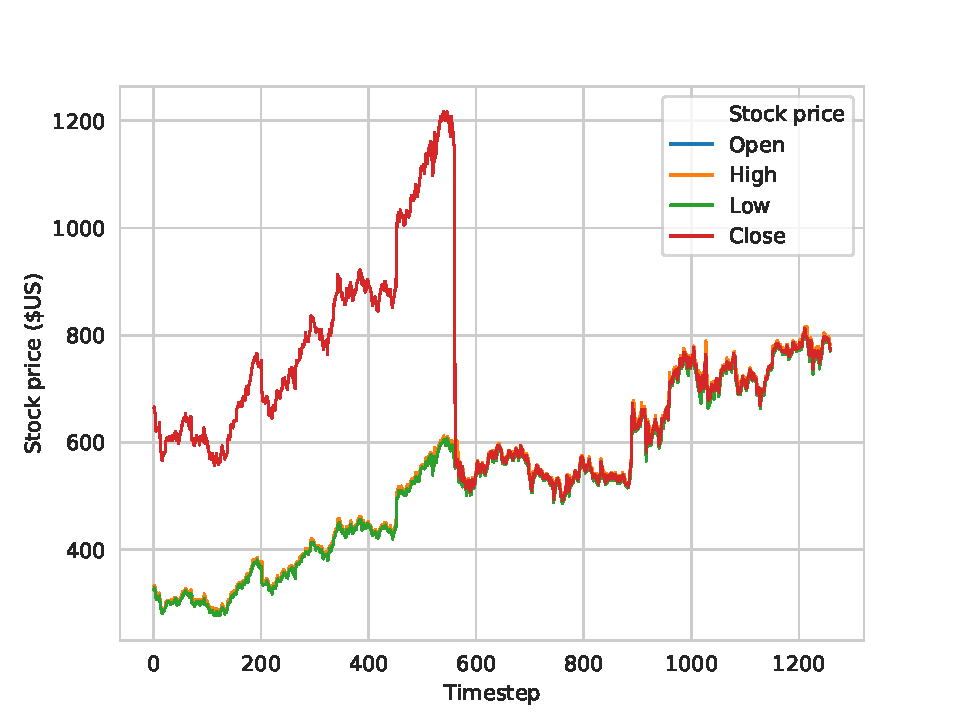
\includegraphics[width=1.0\linewidth]{stock_price.pdf}
	\end{center}
	\caption{Open, High, Low and Close prices of the Google stock (uncorrected)}
	\label{fig:price}
\end{figure}

As seen in other implementations of deep learning for stock price prediction \cite{Zhao2020,Kara2011}, the stock prices were rescaled using minimum maximum normalization to leave the stock prices from 0 to 1, using the following equation:

\begin{equation}
	x' = (b-a) \times \frac{x - min(x)}{max(x)-min(x)} + a
\end{equation}

where $b$ is the new maximum (in this case +1), $a$ in the new minimum (0), $x$ is the original feature and $x'$ is the transformed feature.

\subsubsection{Sliding window}

The prediction of stock price data is usually performed using a sliding window or "look back" representation of the data. This means that the data used as input to predict the near future comes from the closest $N$ days (usually around 20-30), as the data far away from the target usually does not provide useful information for the prediction \cite{Saud2020}.

To use this approach, a sliding window approach was implemented, generating sets of explanatory variables comprising the $N$ days before the target data, and matching them with the target variable day, including the Open, Low, High and Low prices, along with the trading Volume. For practical purposes, the Date field was neglected, and only the days with available records were considered as part of the sliding window.

\subsection{Gated Recurring Unit Neural Network}

To predict the stock prices, a neural network comprised of Gated Recurring Units (GRU) was used. The GRU is comprised by two gates (reset and update), that contribute to the output ( graphical details in Figure \ref{fig:gru}). On one side, the reset gate ($r_t$) is calculated as follows \cite{Chung2014}.

\begin{equation}
	r_t = \sigma (W_r x_t + U_r h_{t-1} + b_r) 
\end{equation}

where $x_t$ is the input data for time $t$, and $h_{t+1}$ is the previous hidden state, while $W_r$ and $U_r$ are set of weights of the gate, and $b_r$ is the bias term.

While, similarly, the update gate ($z_t$) is calculated as follows:

\begin{equation}
	z_t = \sigma (W_z x_t + U_z h_{t-1} + b_z) 
\end{equation}

The candidate hidden state ($\tilde{h_t}$) is calculated as:

\begin{equation}
	\tilde{h_t} = tanh(W x_t + U (r_t \odot h_{t-1} + b_z) 
\end{equation}

Finally, the output of the GRU ($h_t$) is calculated as a result of the previous output ($h_{t-1}$) and the candidate hidden state ($\tilde{h_t}$).

\begin{figure}[h]
	\begin{center}
		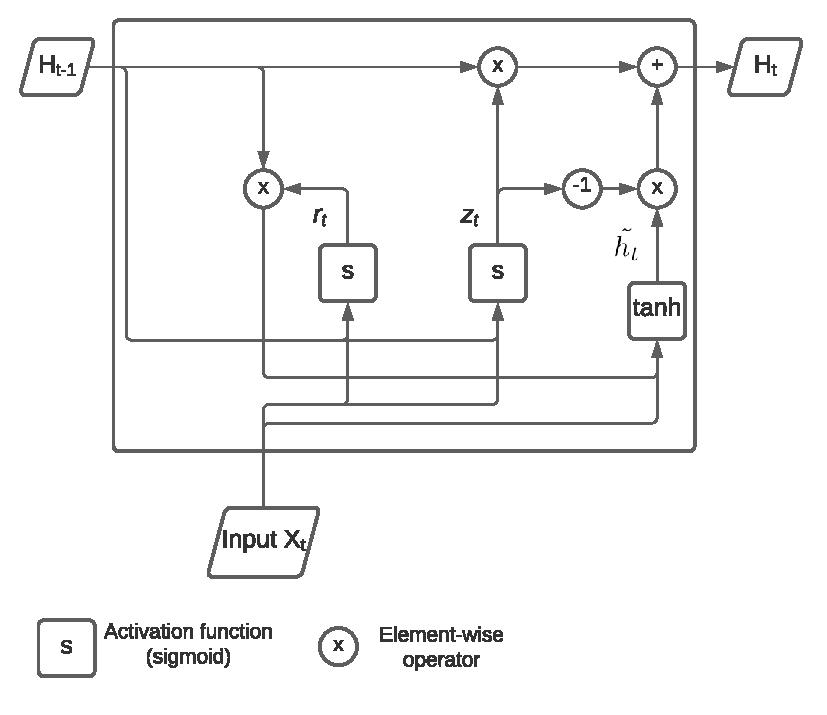
\includegraphics[width=1.0\linewidth]{GRU.pdf}
	\end{center}
	\caption{Gated Recurring Unit neural network architecture used in this study}
	\label{fig:gru}
\end{figure}

To form a neural network from the GRU, the architecture represented in Figure \ref{fig:gru_nn} was implemented. It that figure it is possible to appreciate that the input data (Open, Low, High and Close prices, along with the traded volume) as a sequence is used to feed the neural network, this data is processed by multiple GRU units in the hidden layer, the output of these units is then directed to a fully connected layer, that produces five outputs (Open, Low, High, Close and Volume).

\begin{equation}
	h_t = (1-z_t) h_{t-1} + z_t \tilde{h_t}
\end{equation}

\begin{figure}[h]
	\begin{center}
		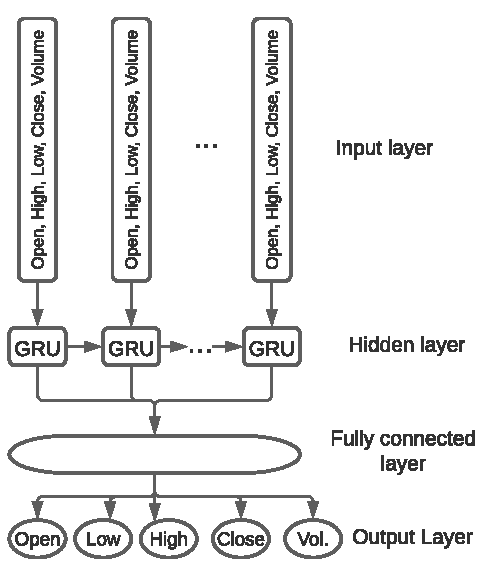
\includegraphics[width=1.0\linewidth]{GRU_nn.pdf}
	\end{center}
	\caption{Gated Recurring Unit neural network architecture used in this study}
	\label{fig:gru_nn}
\end{figure}

\subsection{Loss function and optimization criterion}

In order to train the neural network, a Mean Square Error (MSE) loss function was used:

\begin{equation}
	MSE = \frac{1}{n}\sum_{i=1}^{n} (y_i - \hat{y}_i)^2
\end{equation}

where y is the predicted stock price and $\hat{y}$ the true data

Using this loss function, backpropagation was used to update the parameters of the neural network, for the this purpose, the Adam optimizer was applied. The Adam optimizer was introduced by Kingma and Ba \cite{Kingma2015} and provides a computationally efficient method for stochastic optimization suitable for noise and sparse gradients. This optimizer is often used in the training of recurrent neural networks \cite{Zhao2020}.

\subsection{Hyperparameter tuning}

In order to increase the prediction performance of the neural network, several hyperparameters were tuned. To perform this, a validation set was created using the 20 last records of the training set (the same length as the test dataset). Using grid search (testing all the possible combination of parameters), the prediction performance of the neural network was tested on this validation dataset, and the MSE was calculated. The set of parameters with the smaller MSE was then selected for the final model.

In Table \ref{table:tuning} it is possible to see that one of the tunes hyperparameters (window size) belongs to the preprocessing of the data, while the other parameters belong to the architecture of the neural network (hidden layer size, number of recurrent layers) and to the training process (number of epochs and learning rate)

\begin{table}[H]
	\begin{center}
		\begin{tabular}{|p{4.2cm}|p{3cm}|}
			\hline
			Hyperparameter & Values \\
			\hline\hline
			Window size & 20, 30, 40\\
			Hidden Layer Size & 20, 30, 40\\
			Number of recurrent layers & 1, 2, 3 \\
			Number of epochs & 500, 1000, 1500\\
			Learning rate & 0.01, 0.05, 0.001\\
			\hline
		\end{tabular}
	\end{center}
	\caption{Parameter tuning}
	\label{table:tuning}
\end{table}

\subsection{Next day and intra day prediction}

In order to test different input/output features and to increase the usability of the predictions of the neural network, three slightly different neural networks configurations were tested. Firstly, the five features of the dataset were used as input and output (as in Figure \ref{fig:gru_nn}), and the values of these features were predicted on the next day after the last observation on the input data (this model will be called \textit{nextday}). Secondly, the same architecture was tested removing the traded Volume from the input and output data, as Wang \textit{et al} \cite{Wang2003} point out that the inclusion of this variable does not help in the prediction of the Stock Price (this model will be called \textit{nextday w/o Volume}). 

Finally, as the trading operations are performed when the particular stock market is open (in practice, between the Open and Close prices), a third variant, that includes the Open price to predict the Low, High and Close price on the same day was implemented. In this case, the input data consists the Low, High and Close price of the $N$ days before, along with the Open price of the same day and of the $N-1$ days before. This last variant was developed to increase the usability of the models, as it can improve the trading decision making information during the day, as having the Low, High and Close prices can help the trader decide to buy or sell the stock before the end of the day (this model will be called \textit{intraday}).

The performance of the models will be evaluated using the Root Mean Square Error (RMSE) metric on the test data, using the original scale of the data, using an error metric that is in the same unit as the variable itself, and it is commonly used as an error metric in the field \cite{Qiu2020,Sethia2019}

\begin{equation}
	RMSE = \sqrt{\frac{1}{n}\sum_{i=1}^{n} (y_i - \hat{y}_i)^2}
\end{equation}
 
\section{Code and processing}

The code, along with the requirements and setup instructions for the reproduction of the above-mentioned method, can be found in the following GitHub repository: \url{https://github.com/juliancabezas/RNN-GoogleStockPrice}. All the processing was performed in a Linux OS with NVIDIA GeForce GTX 1050 with CUDA support.

\section{Results and discussion}



\subsection{Data correction}

The correction of the Close price resulted in the prices shown in Figure \ref{fig:price_corrected}, where is it possible to see that in the long term, the Google stock prices tends to increase its price, but showing several price drops in between. Looking at the data, it is also possible to appreciate that the four prices are relatively close to each other, not showing large intraday variations. 

\begin{figure}[h]
	\begin{center}
		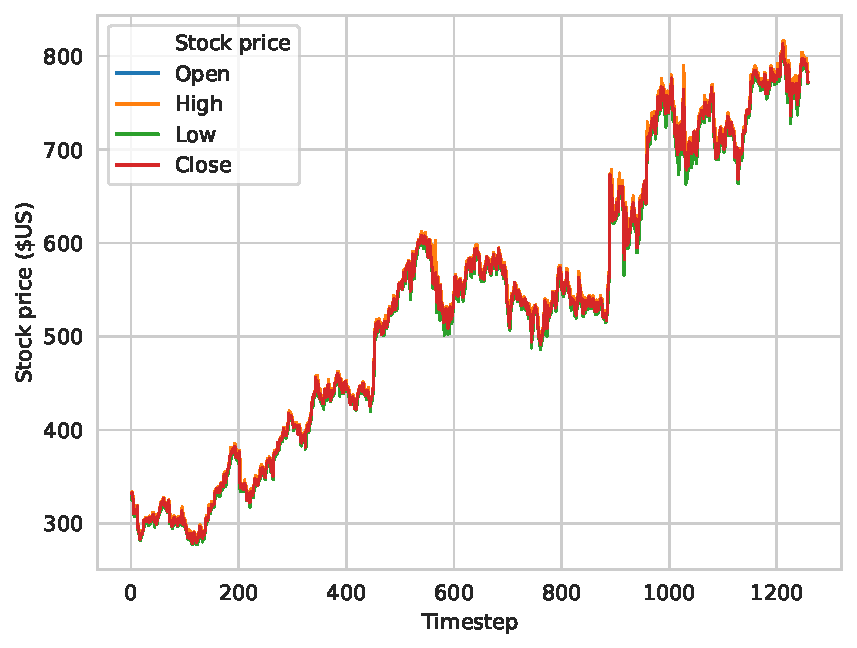
\includegraphics[width=1.0\linewidth]{stock_price_corrected.pdf}
	\end{center}
	\caption{Open, High, Low and Close prices of the Google stock (corrected)}
	\label{fig:price_corrected}
\end{figure}

On the other hand, as seen in Figure \ref{fig:volume}, the trading volume presents an unpredictable and noisy behaviour, with several spikes in trading.

\begin{figure}[h]
	\begin{center}
		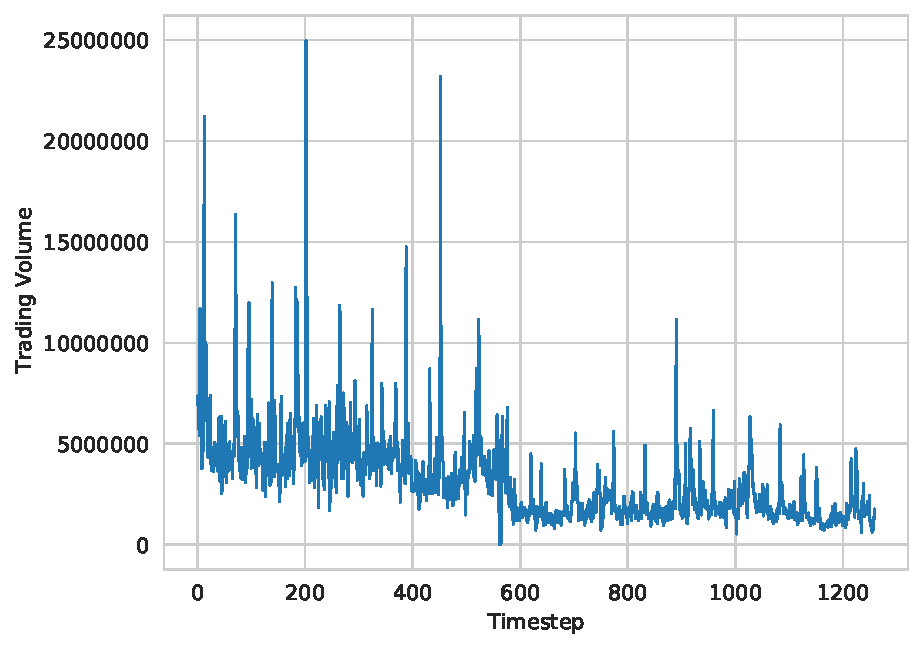
\includegraphics[width=1.0\linewidth]{volume.pdf}
	\end{center}
	\caption{Trading volume of the Google stock}
	\label{fig:volume}
\end{figure}

\begin{figure*}[h]
	\begin{center}
		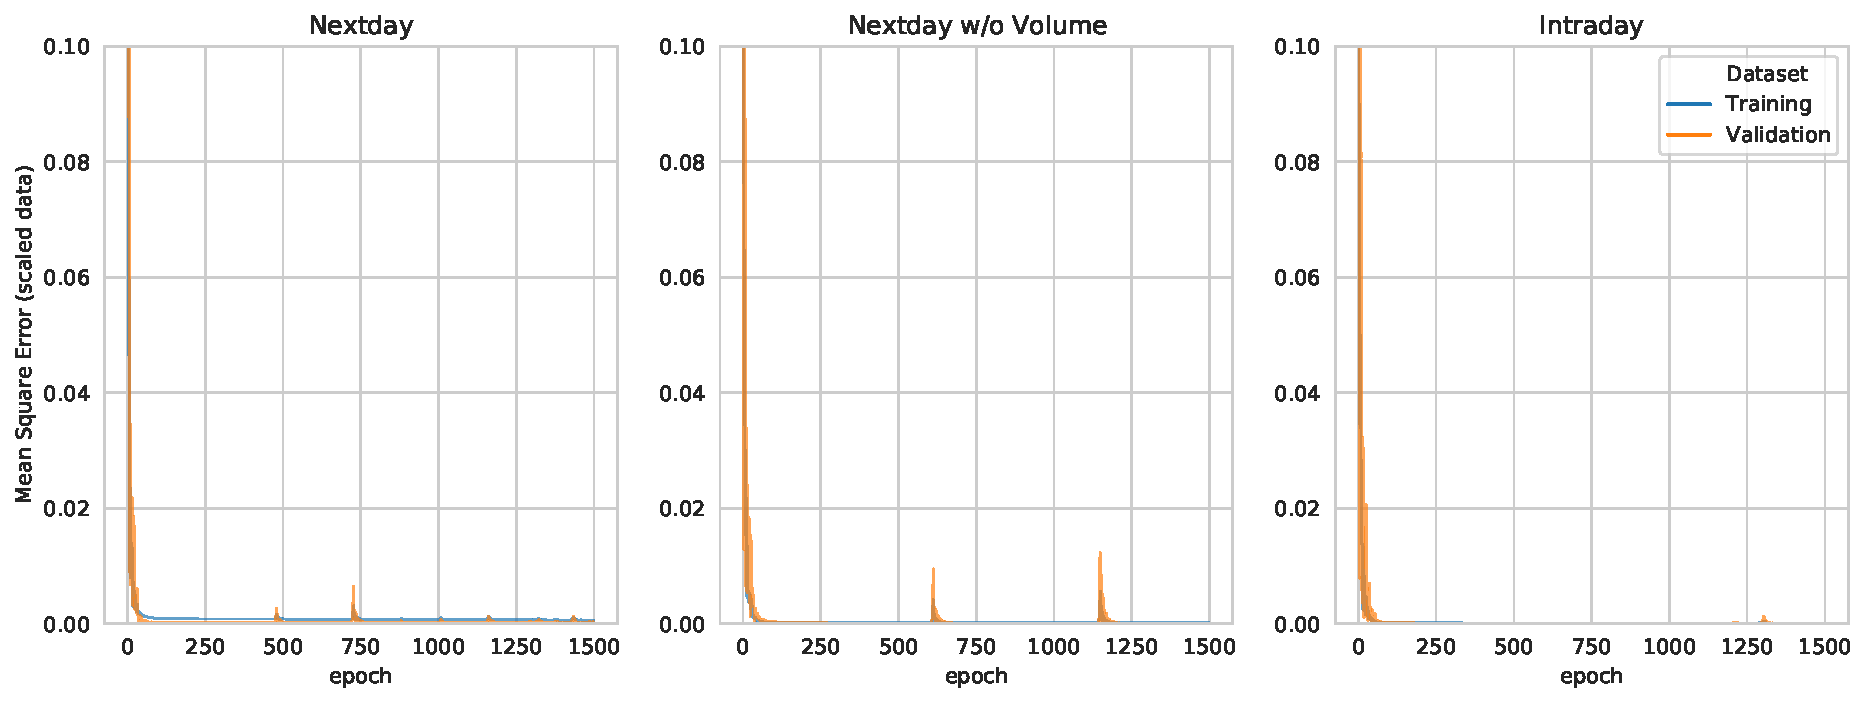
\includegraphics[width=1\linewidth]{train_val_loss.pdf}
		\caption{Training and validation loss (MSE) curves for the three tested models}
		\label{fig:loss}
	\end{center}
\end{figure*}

\subsection{Hyperparameter tuning}

The hyperparameters of the three models (\textit{nextday}, \textit{nextday w/o volume} and \textit{intraday}) were tested, showing the results of Table \ref{table:tuning_res}. It is possible to see that the \textit{nextday} models share the same neural network hyperparameters, but with the \textit{nextday w/o volume} model presenting a smaller window size. On the other side, the \textit{intraday} model seems to benefit with a more complex architecture, presenting a larger hidden layer size (40) and two recurrent layers. All the models achieve better performance with the maximum amount of epochs tested (1500).

\begin{table}[H]
	\begin{center}
		\begin{tabular}{|p{2.9cm}|p{1cm}|p{1.3cm}|p{1.1cm}|}
			\hline
			Hyperparameter & Nextday & Nextday w/o vol. & Intraday \\
			\hline\hline
			Window size & 40 & 30 & 40 \\
			Hidden Layer Size & 30 & 30 & 40 \\
			Number of recurrent layers & 1 & 1 & 2 \\
			Number of epochs & 1500 & 1500 & 1500 \\
			Learning rate & 0.05 & 0.05 & 0.01 \\
			\hline
		\end{tabular}
	\end{center}
	\caption{Parameter tuning results for the three tested models}
	\label{table:tuning_res}
\end{table}

\subsection{Training and testing of the final models}

Using the tuned hyperparameters, the three models were trained using 1500 epochs. In Figure \ref{fig:loss} it is possible to see that the loss (Mean Square Error) on the training and validation data tends to drop consistently, without showing signs of overfitting.

\begin{figure}[h]
	\begin{center}
		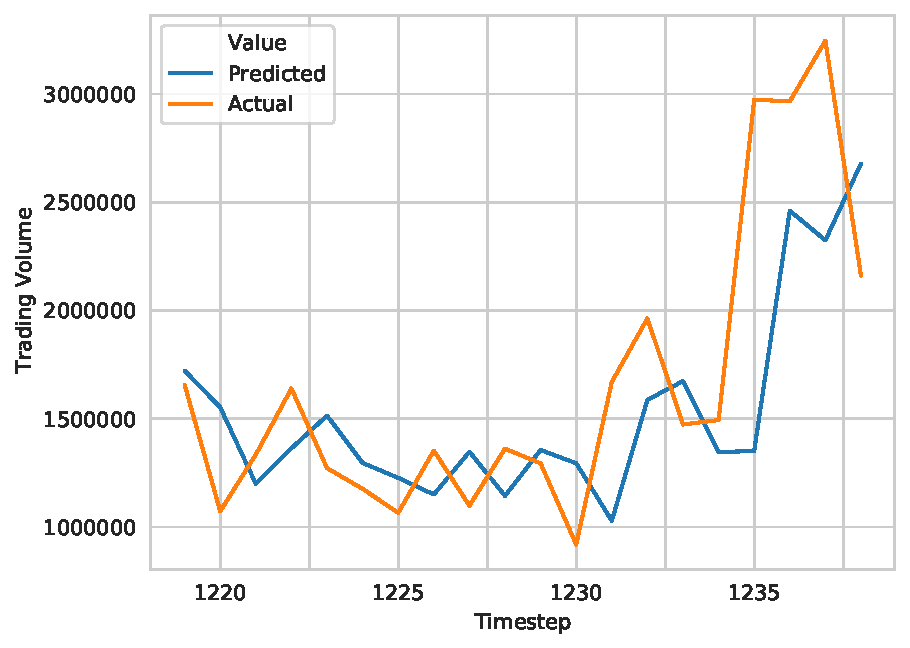
\includegraphics[width=1.0\linewidth]{prediction_volume.pdf}
	\end{center}
	\caption{Test data prediction of the trading volume of the Google stock (\textit{nextday} model)}
	\label{fig:volume_pred}
\end{figure}

The performance of the three models on the test data is shown in Table \ref{table:error}. In that table, it is possible to see that, in the three models, the training error is significantly smaller than the test error, showing a poor generalization of the models. The \textit{nextday} model presents large errors in all the price predictions, with RMSE ranging from 5.96 in the Open price to 8.31 in the Close price prediction. When removing the Volume variable from the input and output of the neural network (\textit{nextday w/o volume} model), the test error of the price predictions is slightly reduced. This results are consistent with the ones reported by Wang et al \cite{Wang2003}, that determined that the inclusion of the volume can slightly increase the test error of the stock price prediction. Thus, the trading volume, at leat in this case, seems to not contain useful information for price prediction. 


\begin{table*}[h]
	\begin{center}
		\begin{tabular}{|p{1.8cm}|p{2cm}|p{2cm}|p{1.8cm}|p{1.8cm}|p{1.8cm}|p{1.8cm}|}
			\hline
			& \multicolumn{2}{c}{Nextday} & \multicolumn{2}{c}{Nextday w/o volume} & \multicolumn{2}{c|}{Intraday} \\
			\hline
			Variable & Train RMSE & Test RMSE & Train RMSE & Test RMSE & Train RMSE & Test RMSE \\
			\hline\hline
			Open price & 2.8498 & 5.9382 & 1.5054 & 5.5476 & - & - \\
			Low price & 2.6912 & 6.8495 & 2.2645 & 6.6231 & 1.8879 & 3.9610\\
			High price & 3.7242 & 6.9893 & 2.6478 & 6.8147 & 1.9452 & 4.5980 \\
			Close price & 2.9339 & 8.3147 & 2.9052 & 8.1642 & 2.4615 & 6.3192 \\
			Volume & 954948.9845 & 1314561.2588 & - & - & - & - \\
			\hline
		\end{tabular}
	\end{center}
	\caption{Error of the models (RMSE) in the train and test dataset}
	\label{table:error}
\end{table*}

The volume prediction presents a very high error in the only model that is included (\textit{nextday}), with an RMSE of 1314561.26 in the test data, and Figure \ref{fig:volume_pred}
 shows that the volume prediction seems to be shifted and inaccurate, showing the difficulties of predicting the trading volume.


\begin{figure*}[h]
	\begin{center}
		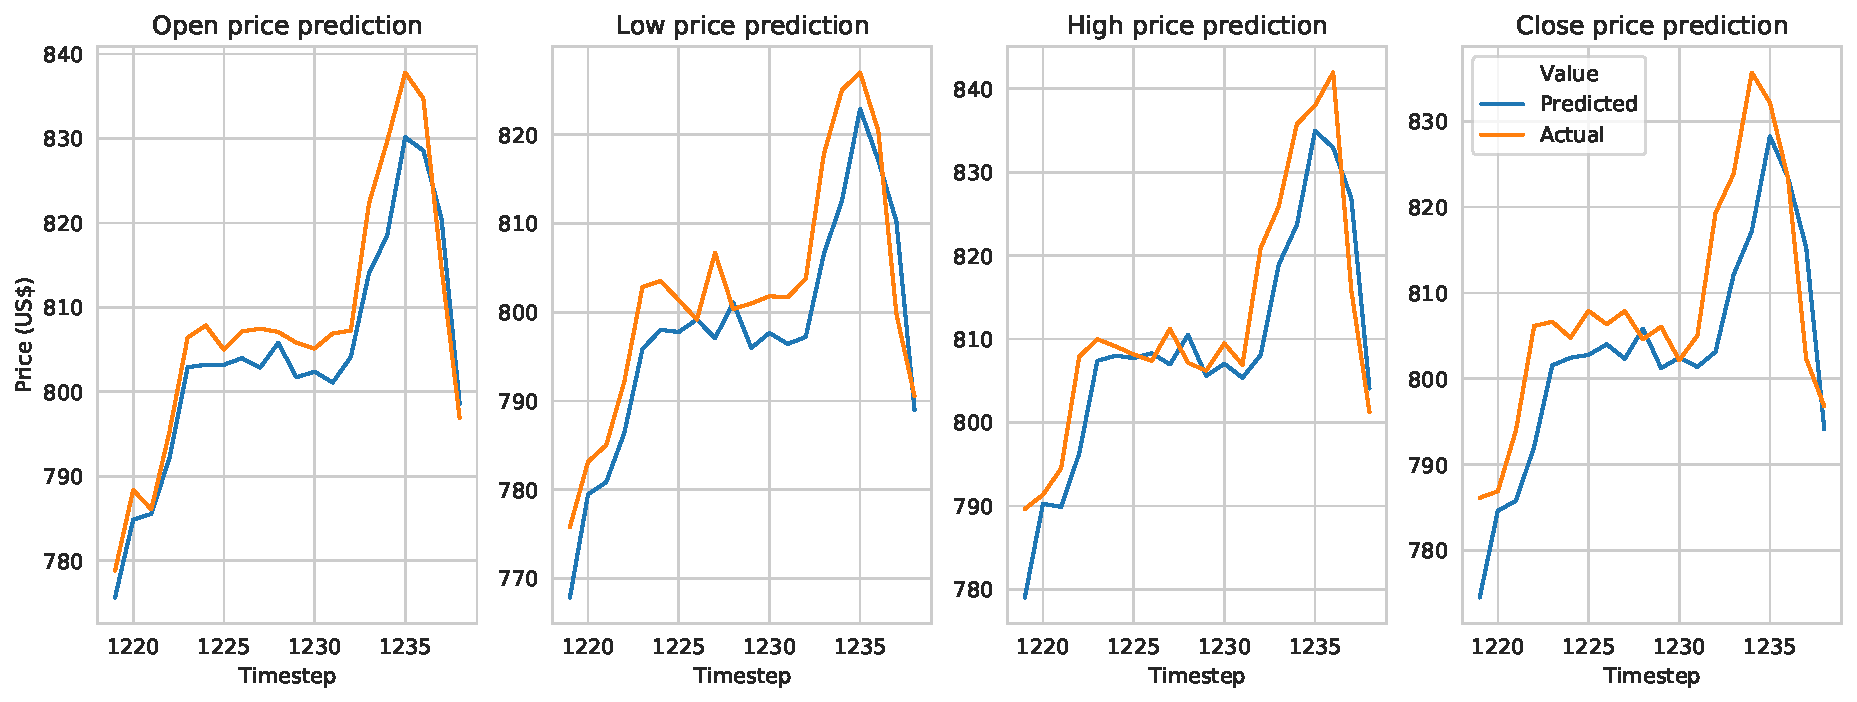
\includegraphics[width=1\linewidth]{prediction_nextday.pdf}
		\caption{Prediction of the \textit{nextday} model for the test data}
		\label{fig:nextday_pred}
	\end{center}
\end{figure*}

\begin{figure*}[h]
	\begin{center}
		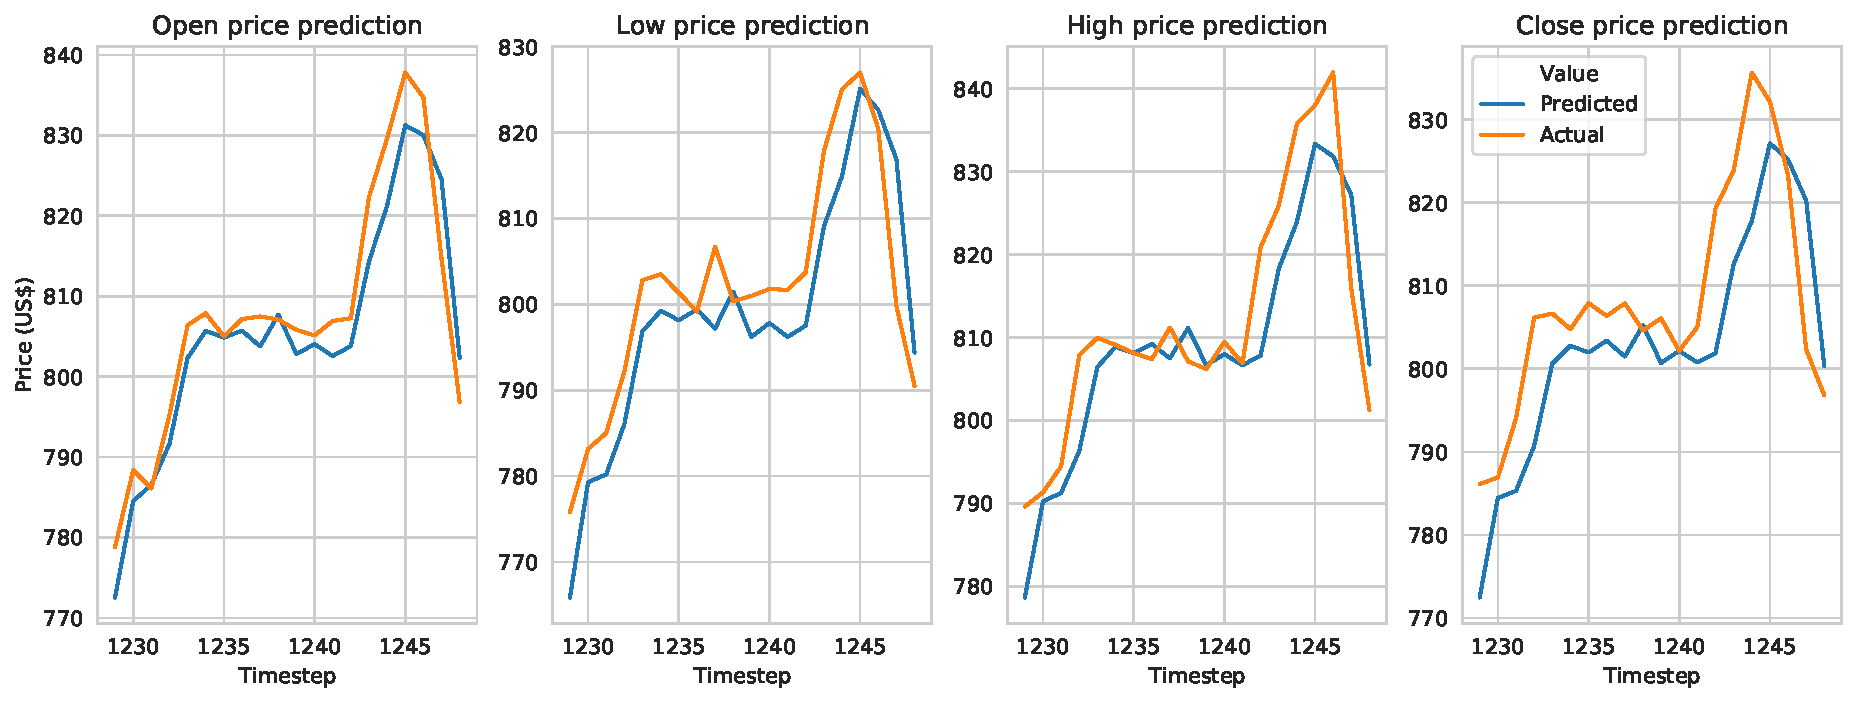
\includegraphics[width=1\linewidth]{prediction_nextday_novolume.pdf}
		\caption{Prediction of the \textit{nextday w/o volume} model for the test data}
		\label{fig:nextday_novolume_pred}
	\end{center}
\end{figure*}


In Figures \ref{fig:nextday_pred} and \ref{fig:nextday_novolume_pred}, it is possible to see that the prediction for the nextday models is in general shifted one day or time-step away from the actual data, showing that the model mostly uses the data from the previous day to predict the future behaviour of the price. Given this information, the nextday models could not be considered for use in a real-life scenarios, and could lead to late decision in trading.

On the other side, when analysing the \textit{intraday} model results (Table \ref{table:error}), it is possible to see that the inclusion of the Open price of the same day of the prediction greatly increases the performance of the models, both in the training and testing for the Low, High and Close Prices. In the case of the Low price, the RMSE goes from 6.62 in the nextday model without volume to 3.96 in the intraday model, with the High and Close prices showing similar reductions in the error. These results are relevant for the usability of the model, as in general the trading operations are performed during the day, thus, the trader already knows the Open price when he/she is deciding to make a trading operation, making the intraday model suitable to be used at the beginning of the day to help the decision making process of the trader. 

When looking at the predicted values in the test data, the \textit{intraday} model seems to predict the behaviour of the Low, High and Close prices more accurately, with special emphasis on the Low price (Figure \ref{fig:intraday_pred}), that shows a very close to the actual price prediction at the end of the test data, where a drop in price occurs.

In order to asses the usability of the \textit{intraday} in a real world situation, it is possible to compare the error values with the price variations of the Google Stock during the day. Looking a the test data, it is possible to calculate that the mean difference between the Low and High price is 9.97 USD, with a minimum difference of 4.53 and a maximum difference of 21.51 USD. This values contrast with the RMSE of the Low and High prediction, that are 3.96 and 4.60 USD respectively, making this model useful as an input of the decision making for operations inside trading hours, as it can provide useful information about the possible High and Low prices of the Google stock, possibly helping traders increase their profit \cite{Naik2020}.


\begin{figure*}[h]
	\begin{center}
		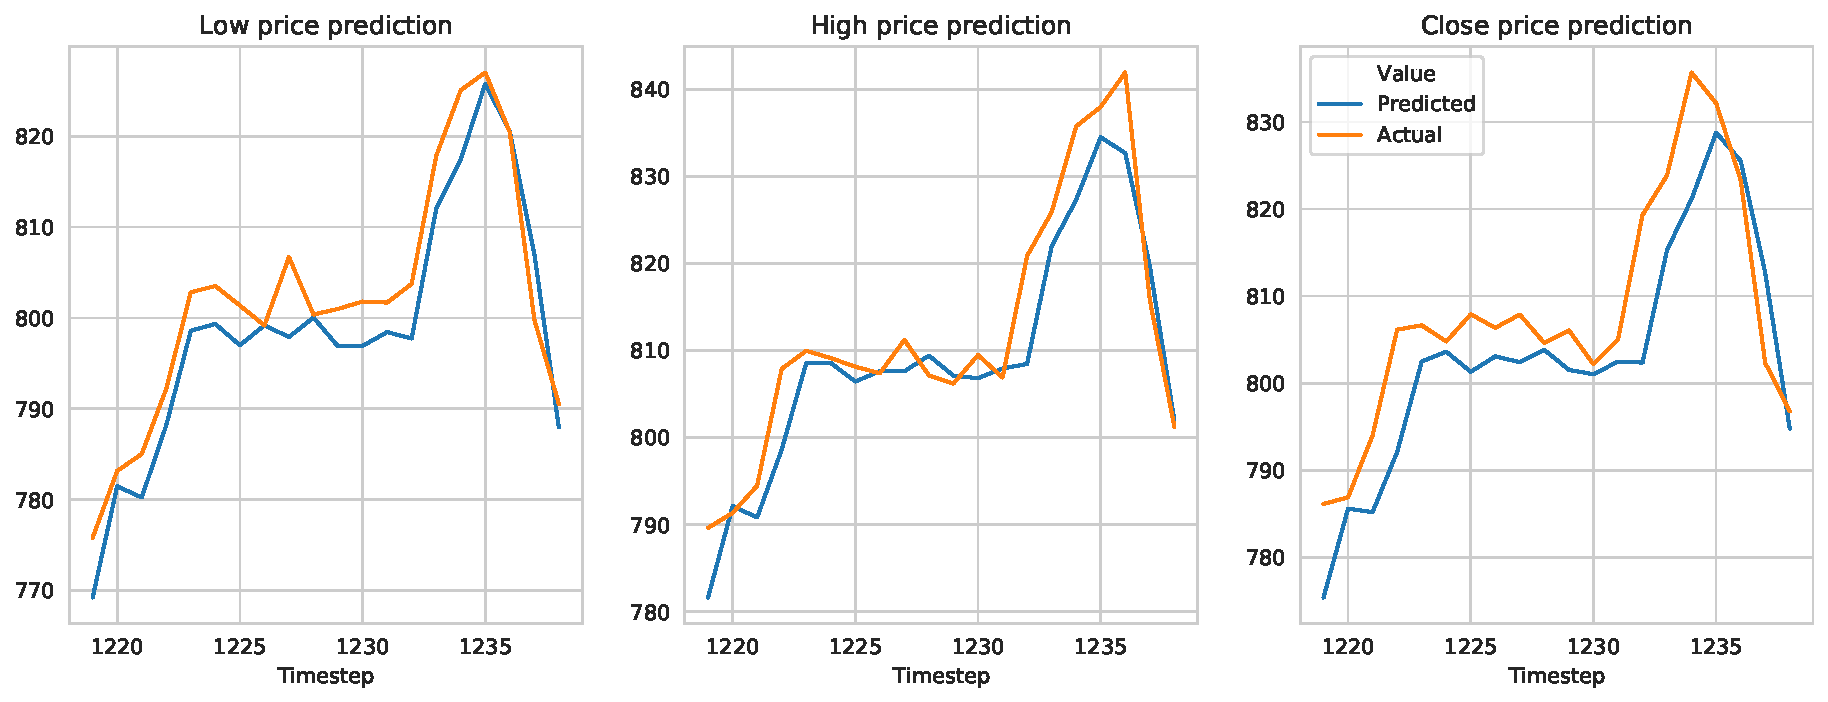
\includegraphics[width=0.9\linewidth]{prediction_intraday.pdf}
		\caption{Prediction of the \textit{intraday} model for the test data}
		\label{fig:intraday_pred}
	\end{center}
\end{figure*}

Despite the acceptable results in performance shown in this paper, the use of this model as sole input for trading operations has to be discouraged, as in big trading operations, a prediction error of the magnitude achieved in this research can cause losses of millions of dollars for the trader. Moreover, the price of a particular stock can be influenced by several factors that are not taken into account in this research, such as price sensitive news announcements \cite{Mazouz2015} and macro economical conditions, ranging from political events to firms policies \cite{Tan2007}

\section{Conclusion}

This research shows that the use of GRU neural networks, provided enough hyperparameter tuning and a correct choosing of input and output variables, can provide acceptable predictions of the stock price in the future, that can be useful to aid the decision making process of the stock traders, but that has to be complemented with the experience of the trader itself and considering possible external factors that can influence these values. 
In the future, variables such as other stock prices, news appearance and other factors can be included to improve the performance of the model, as well as to consider the inclusion of attention mechanisms in the implemented neural networks to increase the performance of the model itself, as seen in the latest literature on RNN. Finally, even though efforts were done to improve the performance of the tested models, this research also confirms stock price predictions as one of the biggest challenges in time series prediction.

\section{Bonus}

This research provided insight over the importance of including the Open price in order to increase the usability of the models, showing great difference between models that generate predictions for the next over models for intraday prediction. This research also confirms the hypothesis of Wang \textit{et al} \cite{Wang2003}, verifying that in this case the trading volume does not help in the prediction of stock prices, mainly due to the noisy nature of the variable.

{\small
\bibliographystyle{ieee_fullname}
\bibliography{library}
}

\end{document}
